\documentclass{article}
\usepackage{amssymb,amsfonts,amsmath,calc,tikz,geometry}
\usepackage{color}   %May be necessary if you want to color links
\usepackage{hyperref}
\hypersetup{
    colorlinks=false, %set true if you want colored links
    linktoc=all,     %set to all if you want both sections and subsections linked
    linkcolor=black,  %choose some color if you want links to stand out
}
\geometry{margin=1in}
\newcommand{\N}{\mathbb{N}}
\newcommand{\Z}{\mathbb{Z}}
\newcommand{\Q}{\mathbb{Q}}
\newcommand{\R}{\mathbb{R}}
\newcommand{\Omicron}{O}
\newtheorem{thm}{Theorem}[section]

\title{\textbf{Set Theory I}}
\author{Yeheli Fomberg}
\date{}

\usepackage{amsmath}
\begin{document}
	\maketitle
	\newpage
	\tableofcontents
	\newpage
	\section{Permutations}
		Permutation $\sigma$ is a bijection from a set $S$ onto iteself. \\
		Every permutation can be decomposed into one or more disjoint cycles(or orbits), thus, they can also be defined by them like this:
		\begin{center}
			$\sigma=$
				$\begin{pmatrix}
					1 & 2 & 3 & 4 & 5\\
					2 & 5 & 4 & 3 & 1\\
				\end{pmatrix}$
			=$(3 \ 4)(1 \ 2 \ 5)$
		\end{center}
		\begin{enumerate}
			\item A cycle of one element is call a \textbf{fixed point}
			\item A permutation without fixed points is called a \textbf{derangement}
			\item A permutation that's an orbit of 2 elements is called a \textbf{transposition}
		\end{enumerate}
		
		\subsection{The symmetric group}
		A symmetric group defined over a set is the group whose elements are all the permutation over the set, and whose group operation is the composition of functions. \\\\
		Reminder: A group is an algebric structure with the following characteristics:
		
		\begin{itemize}
			\item Associativity
			\item An Idenentity permutation exists
			\item $\forall \sigma \in S_n(\exists\pi:\sigma\circ\pi=Id)$
		\end{itemize}
		
		
	\newpage
	\section{Hall's theorem}
		\textbf{Hall's theorem - } \emph{In a finite bipartite graph 			$G(X,Y,E) \\ \forall W\subseteq X(|W|\le|N_g(W)|)\iff $ An $X$-perfect matching exists.}\\\\
		$(\Leftarrow)$ Suppose we have an $X$ perfect matching $M$, since for any given $W$ all vertices in $W$ have a distinct matching vertice in $Y$ by $M$ we get
		\[\forall W\subseteq X(|W|\le|N_g(W)|)\]
		$(\Rightarrow)$ We'll prove by contradiction. Assume an $X$-perfect matching doesn't exist, we'll denote the maximal matching $M$,and the sets of vertices in $X,Y$ that appear in $M$ as $S,T$.
		An X-perfect matching doesn't exist $\Rightarrow X\setminus S\neq\emptyset$, so we can choose a vertice $u_0\in X\setminus S$ and consider all alternating paths of the form $P=(u_0,v_1,v_2,\ldots)$ such that odd edges are not in $M$ and even edges are in $M$.
		Denote: \[A=\{u:u\in P \land u\in X\} ,\quad B=\{v:v\in P \land v\in Y\}\]
		We know every vertice in $B$ is matched by $M$ to a vertice in $A$ because otherwise we could create a bigger matching by toggling whether each of the edges belong to $M$ or not.
		\[\Rightarrow |B|\le|A\setminus \{u_0\}| \Rightarrow |B|<|A|\]
		but also for any vertice in $a\in A$ any of its neighbors $b$ are in $B$. We can show that an alternating path to $b$ exists either by removing the matched edge $ab$ from the alternating path to $a$, or by adding the unmatched edge $ab$ to the alternating path to $a$.
		\[\Rightarrow B=N_g(A) \] \[\Rightarrow |N_g(A)|<|A|\] 
		That's a contradiction so an $X$-perfect matching must exist.
		
\newpage
	\section{Cantor's theorem}
		\[|A|<|P(A)|\]
		We can define $f:A\rightarrow P(A)$ as such
		\[f(a) = {a}\]
		\[\Rightarrow |A|\le|P(A)|\]
		Assume $|A|=|P(A)|$. That means there's a bijection $g:A\rightarrow P(A)$. \\
		consider the following set:
		\[D = \{a:a\notin g(a)\}\]
		Since $g$ is a bijection $\exists b\in A:f(b)=D$. Now look at the different cases:
		\[
		\begin{cases}
		b\in D, & b\notin g(b)=D \Rightarrow contradiction\\
		b\notin D=g(b), & b\in D \Rightarrow contradiction
		\end{cases}
		\]
		Therefore $|A|\neq|P(A)| \Rightarrow |A|<|P(A)|$
		
		
\newpage
	\section{Equivalence Relations}
	An equivalence relation is a binary relation (a set of ordered pairs) that is
	\begin{itemize}
	\item Reflexive
	\item Symmetric
	\item Transitive
	\end{itemize}
	
	\subsection{Some Terminology}
		Suppose we have an equivalnce relation $R$ on a set $X$:\\\\
		\textbf{Equivalence Class:} $[a]_R = \{b\in X:bRa=1\}$\\
		\textbf{Quotient Set:} $X/R = \{[a]_R:a\in X\}$\\
		\textbf{Projection:} The projection of $R$ is $\pi:X\rightarrow X/R$ such that $\pi(x)=[x]_R$\\
		\textbf{A Cut:} A cut of $X$ is a set with only one element of each Equivalence class.\\\\
		Equivalence relations can be defined by their Quotient set.
Thus they can also be defined by a function or a partition.
		The numbers of partitions of a set $|X|=n$ are known as Bell's numbers and can be calculated recursivly as such: $$B_{n+1}=\sum_{k=0}^{n}{n\choose k}B_k$$\\
		Think why.
		
\newpage
\section{Kőnig's Theorem}
	\textbf{Kőnig's Theorem - } \emph{For an index set $I$, suppose$\,\,\forall i\in I$ and $\kappa_i,\lambda_i$ we know $\kappa_i<\lambda_i$} then $\sum_{i\in I}\kappa_i<\prod_{i\in I}\lambda_i$\\
	We'll show this by proving for any
	\[f:\sum_{i\in I}B_i\rightarrow \prod_{i\in I}C_i \quad |B_i|=\kappa_i, |C_i|=\lambda_i\]
	That $f$ is not surjective.
	Let's define the function $f_i$ as such:
	\[f_i:B_i\rightarrow C_i\]
	\[f_i(x)=f(x)_i\]
	$\forall i\in I(|B_i|<|C_i|)\Rightarrow \forall i\in I(f_i$ is not surjective) $\Rightarrow \exists c_i\in C_i\setminus Imf_i$ \\
	Consider the vector: $$\hat{c} = \ <c_i:i\in I>$$
	If $\hat{c}\in Imf \Rightarrow \exists i\in I,b\in B_i:f(b)=\hat{c}$\\
	$\Rightarrow f(b)_i=c_i \Rightarrow f_i(b)=c_i$ but $c_i\in C_i\setminus Imf_i$\\
	That's a contradiction so we got \[|\sum_{i\in I}B_i|< |\prod_{i\in I}C_i| \Rightarrow \sum_{i\in I}\kappa_i<\prod_{i\in I}\lambda_i\]

\newpage

\section{Partial Orders}
A \textbf{Weak/Non-Strict} Partial Order is a homogeneous relation $\le$ on a set $P$ that is:
\begin{itemize}
\item Reflexive
\item Antisymmetric \footnote[1]{$a\le b \land b\le a \Rightarrow a=b$}
\item Transitive
\end{itemize}
A \textbf{Strong/Strict Partial} Order is a homogeneous relation $<$ on a set $P$ that is:
\begin{itemize}
\item Irreflexive
\item Asymmetric\footnote[2]{$a<b \Rightarrow \lnot b<a$}
\item Transitive
\end{itemize}
note: $<\bigcup\le_{Id}=\le$
\section{Partially Ordered Sets}
A Partially Ordered Set(aka a poset) is a set on which a partial order is defined $(A,\le).$ We say
two elements $a,b\in A$ are comparable $\iff a\le b\lor b\le a$\\
If two elements are incomparable they're linearly independent.
A \textbf{linear/total order} is a partial order under which every pair of elements is comparable. All ordered subsets(chains) are linearly independent of each other.
\subsection{Extrema}
\textbf{Greatest Element} - \emph{an element that's comparable and greater than all other elements}\\
\textbf{Maximal Element} - \emph{an element that doesn't have a greater element than him}\\
\textbf{Upper/Lower Bounds in sets} - \emph{a is a bound in $A$ of $B\subseteq A$ if $a\in A \land \forall b\in B(b\le a)$}
\subsubsection{About Lattices}
Let A be a partially ordered set:\\
    $A$ is a lattice $\iff \forall S\subseteq A(|S|=2 \Rightarrow SupS,InfS \quad\text{exist})$
    
\newpage
\section{Cardinals}
Cardinal numbers are the "numbers" we use to represent the cardinality of sets. Their "size".
All cardinal numbers are based on the size of $\N$ that is $\aleph_0$.
This subject is rather simple, yet hard to start from scratch.
Thus I encourage you to try to prove the following:

\begin{enumerate}
    \item $|\N|<|\R|$
    \item $\aleph_{0} $ = $\aleph_{0}+n =\aleph_0\times n=\aleph_0\times\aleph_0=|\Z|=|\Q|$
    \item $\aleph = 2^{\aleph_0} = |(0,1)^{\aleph_0}| = \aleph\times\aleph_0 = \aleph\times\aleph = |(0,1)| = |[0,1]|$
    \item A plane can't be covered by $\aleph_0$ lines.
    \item Let A be an infinte set, $\exists S\subseteq A : |S|=\aleph_0$
    \item $\aleph = |P(\N)|= |P(\Q)|$
    \item let A = \{The set of all finite subsets of $\N$\} prove $|A|=\aleph_0$
    \item $\aleph^\aleph_0=\aleph$
    \item $|\R^\R|=|P(\R)|=2^\aleph$
    \item $|$The disjoint union of $\N$ sets of size $\N|$= $\aleph_0$
    \item $\aleph_0^{\aleph_0} =\aleph$
    \item $|$The set of all invertible functions $\R\rightarrow\R|$= $2^\aleph$
    \item $|A|=|$The set of all algebric numbers$|=\aleph_0$
    \item $|B|=|\R\setminus A|=|$The set of all transcedental number$|=\aleph$
    \item $|$All subsets of $\R$ with cardinality $\aleph/\aleph_0|$
    \item Let $\aleph_0$ people with a natural number of hats on their head guess how many hats they have. How many options are there, given only a finite number of people guessed right/wrong?
    
\end{enumerate}


\newpage
\section{Schröder–Bernstein Theorem}
\textbf{Schröder–Bernstein Theorem} - \emph{$|A|\le|B|\land|B|\le|A|\iff|A|=|B|$}
There are more proofs that rely on similiar ideas. Here's one:\\
We're given two injective functions
\[f:A \rightarrow B\]
\[g:B \rightarrow A\]
Without loss of generality assume A,B are disjoint(Why can we do this?)\\
Considering the partially defined functions $f^{-1}, g^{-1}$ we can create a sequence for every element of $A\bigcup B$ in the following way:
$$\ldots f^{-1}g^{-1}(a)\rightarrow g^{-1}(a)\rightarrow a\rightarrow f(a) \rightarrow g(f(a))\ldots$$
The sequence can keep going forever to the right, but to the left it may stop eventually since the inverse functions are partial\footnote[1]{We'll call those who stop from the left on an element of $A$ A-stops and the rest B-stops - even though they may not always stop!}. We can see that every element in $A\bigcup B$ has a sequence and that if an element appears in two sequnces they'll be identical since they're injective and by our construction. Thus those sequences form a partition of $A\bigcup B$ so it's sufficient to create bijections for all partitions, and we're finished. Our bijection will be:\\
\[
    h(x) = \left\{\begin{array}{lr}
        f(x), & \text{for } x\in A\text{ in an A-stop}\\
        g^{-1}(x), & \text{for } x\in A\text{ in a B-stop}\\
        f^{-1}(x), & \text{for } x\in B\text{ in an A-stop}\\
        g(x), & \text{for } x\in B\text{ in a B-stop}\\
        
        \end{array}\right\}
  \]
  And of course any element of an A-stop can go one step right with $f$ and we can get any element's left neighbor by applying $f^{-1}$, and so we get a bijection for any $A$-stop sequence. The proof for $B$-stops is similiar. Finally, we get that $h$ is the bijection we looked for and that $|A|=|B|$.
  
  \newpage
  \section{Homomorphism and Isomorphosm of Ordered Sets}
  \subsection{Homomorphisms}
  Let $(X,\le_1) , (Y,\le_2)$ be partially ordered sets.
\[F \text{ is a Homomorphism} \iff \forall x_1,x_2 \in X(x_1 \le_1 x_2 \Rightarrow F(x_1)\le_2 F(x_2)\]

	\subsection{Isomorphisms}
	  Let $(X,\le_1) , (Y,\le_2)$ be partially ordered sets.
	\[F \text{ is an Isomorphism} \iff F:X\rightarrow Y \text{ is a bijection } \land\, \forall x_1,x_2 \in X(x_1 \le_1 x_2 \Rightarrow F(x_1)\le_2 F(x_2)\]
	An isomorphism is reflexive, symmetric and transitive so it's an equivalnce relation.\\
	If $F$ is an Isomorphism and the orders are total orders, $F^{-1}$ is also an isomorphism.
	
	\subsection{Lexicographic Order}
	Also known as a Dictonary Order, is an order That's defined as such:
\[(x_1,y_1)\le(x_2,y_2) \iff x_1 <_{x} x_2 \lor (x_1=x_2 \land y_1 \le_{y} y_2)\]
This is a partial order on $X\times Y$

\newpage
\section{Zorn's Lemma}
\textbf{Zorn's lemma} - \emph{Let $F$ be a non-empty poset.
If for every chain\footnote{a totally ordered subset} in $F$ exists an upper bound in $F$, then $F$ has at least one maximal element.}
\subsection{Proof All Vector Spaces Have a Base}
Let $V$ be a vector space: If $V=\{0\}$ then $\emptyset$ is its basis. If $V$ is finitely generated then we can add vectors from $V$ to $\emptyset$ until it's spanning $V$.
Suppose $V$ is not finitely generated, let's Define $F$ as the set of all linearly independant sets of vectors.
$F$ is partially ordered by the order of inclusion of sets.
Let $C=(A_i)_{i\in I}$ be a chain in $F$, $A=\bigcup_{i\in I}A_i$. $A$ is clearly a maximal element of the chain. Let's prove it's in $F$.
Assume $A$ isn't in $F$ $\Rightarrow$ there exists a finite series of linearly dependent vectors, each is an element of a finite series of elements of $C$. Since that series is finite, and linearly ordered as a subset of $C$, There exists a maximal element that must contain all the vectors in the linearly independent vector series, but that element is in $F$ so it's both linearly dependent and independent at the same time! contradiction! We get that $A\in F$ so by Zorn's lemma $F$ has a maximal element $T$. That $T$ is our basis.

\subsection{Comparing Cardinals}
We'll show that for every two cardinals $\alpha,\beta$ other than 0 we get $\alpha\le\beta\lor\beta\le\alpha$\\
Let $A,B$ be two sets of cardinality $\alpha,\beta$\
Define F to be the set of all ordered pairs $(X,f)$ such that $f:X\rightarrow B$ is an injective function($X\subseteq A$).
Now we'll define an order in the following way:
\begin{center}$(X_1,f_1)\le(X_2,f_2)\iff X_1\subseteq X_2 \land f_2|_{X_1}=f_1$\end{center}
Let $C=((X_1,f_1),(X_2,f_2),\ldots)$ be a chain in $F$, $(X,g)=(\bigcup A_{i},\bigcup f_i)$
\begin{center}$ \Rightarrow \forall i((X_i,f_i)\le(X,g))$.\end{center}
Assume $g$ isn't a function, we get $(x,y),(x,z)\in G$
\begin{center}$\Rightarrow \exists i,j \text{ such that: } f_i(x)=y,f_j(x)=z$\end{center}
$C$ is a chain so we without lose of generailty we get:
\begin{center}$f_i\le f_j$\end{center}
\begin{center}$\Rightarrow f_j|_{X_i}=f_i$\end{center}
\begin{center}$\Rightarrow f_i(x)=f_j(x)$\end{center}
\begin{center}$\Rightarrow y=z$\end{center}
That means $g$ is a function, and since it's a union of injective functions, it must also be injective. That means it's in $F$ and using Zorn's lemma we get a maximal element in $F$, which we'll denote $(D,h)$. If $D=X$ then $h$ is injective and we get $A\le B$. If it's not, it must be surjective or we get a contradiction to $(D,h)$'s maximality and thus $B\le A$
\\\\
We can also prove $\alpha+\alpha=\alpha$. We know that $\alpha+\alpha=2\alpha$ so we'll just prove $\alpha=2\alpha$. We'll build $F$ using bijections this time. Denote the maximal element $M=(X,g)$. If $|X|=2\alpha$ We finished, else we get that there's a set of size $\aleph_0$ that can be mapped "bijectively" to the set of $2\alpha$ contradicting $M$'s maximality.

\subsection{Corollaries}
\begin{align*}
&\alpha+\beta=max\{\alpha,\beta\} \\
&|A\setminus B|=|A| \iff |B|\le|A| \\
&\alpha*\alpha=\alpha (not a direct corollary) \\
&\alpha^\alpha=2^\alpha \\
\end{align*}
\section{Axiom of Choice}
First let's define what is a choice function. A Choice Function - is a function from an indexed family of sets $(S_i)i\in I$ to their union such that $\forall i\in I(f(S_i)\in S_i)$. Now for the axiom itself,
The Axiom of Choice:
\[
\forall X[\emptyset\notin X \Rightarrow \exists f:X\rightarrow\bigcup X \ \forall A\in X(f(A)\in A)]
\]

\subsection{Nomenclature}
    \textbf{AC} - \emph{Axiom of Choice}\\
    \textbf{ZF} - \emph{Zermelo-Fraenkel set theory omitting AC}\\
    \textbf{ZFC} - \emph{ZF extended to include AC}

\newpage
\section{More Axioms In ZF}
Axiom of extensionality
\[
	\forall A\forall B(\forall x(x\in A \iff x\in B)\Rightarrow A=B)
\]
Axiom of union
\[
	\forall A \exists B \forall c(c\in B \iff \exists D(c\in D \land D\in A))
\]
Axiom of infinity
\[
	\exists I(\emptyset \in I \land \forall x\in I (x\cup \{x\}\in I))
\]
Axiom of power set
\[
	\forall x \exists y \forall z[z\in y \iff \forall w(w\in z \Rightarrow w\in x)]
\]
Axiom of regularity
\[
	\forall x(x\neq\emptyset \rightarrow \exists y(y\in x \land y\cap x = \emptyset))
\]
Axiom of pairing
\[
	\forall A\forall B \exists C\forall D[D\in C \iff (D=A \land D=B)]
\]
\textbf{Axiom schema of specification} - \emph{any definable subclass of a set is a set.}
\textbf{Axiom schema of replacement} \emph{- the image of any set under any definable mapping is also a set}
\newpage
\section{Measure}
Measure theory is complex and goes well beond what I can show in this section but let's talk about it anyway. A measure is a way to generalize the length, volume, and such for sets. Let $X$ be a set and $\Sigma$ a $\sigma$-algebra over $X$. A set function $\mu$ from $\Sigma$ to the extended real number line is called a measure if
\begin{itemize}
\item $\forall E\in\Sigma:\mu(E)\ge 0$
\item $\mu(\emptyset)=0$
\item $\sigma$-additivity: For all countable collections $\{E_k\}_{k=1}^\infty$ of pairwise disjoint sets in $\Sigma$,
\[
\mu(\bigcup_{k=1}^\infty{E_k})=\sum_{k=1}^\infty{\mu(E_k)}
\]
\end{itemize}
If the condition of non-negativity is dropped then $\mu$ is called a signed measure. The pair $(X,\Sigma)$ is called a measurable space, and the members of $\Sigma$ are called measurable sets. A triple $(X,\Sigma,\mu)$ is called a measure space. A probability measure is a measure with total measure $\mu(X)=1$. A probability space is a measure space with a probability measure.
\subsection{Lebesgue Measure}
Now we have to simplify things so we'll consider only Lebesgue measure of bounded sets on the real number line. First, if the set is of the form $X=(a,b)$ or $X=[a,b]$ and such the measure must satisfy $\mu(X)=b-a$, if $Y=f(X)$ and $f$ is an isometric function then $\mu(X)-\mu(Y)$. Denote $\mathcal{Y}=(Y_i)_{i\in I}$ such that $|I|<\aleph_0$ and $X\subseteq \bigcup_{i\in I}{Y_i}$ and each $Y_i$ is an interval on $R$. Denote $s(\mathcal{Y})$ The sum of lengths of intervals in $\mathcal{Y}$. The outer measure of $X$ is
\[\mu^*(X) = \inf_{\mathcal{Y}}s(\mathcal{Y})\]
And the inner measure is defined with an interval $X\subseteq[a,b]$ and $X'=[a,b]\setminus X$
\[\mu_*(X) = (b-a)- \mu^*(X')\]
It's easy to show that the outer measure is always greater than the inner measure. The Lebesgue measure is defined if they are equal and is equal to
\[\mu_*(X)=\mu^*(X)=\mu(X)\]


\newpage
\section{Well Order}
	A partially ordered set $(X,\le)$ is well ordered
	\begin{center}$\iff$ \end{center}
	\begin{center}$\forall S\subseteq X(S\neq\emptyset\rightarrow \exists b\in S(\text{b is a minimal element is S}))$\end{center}
	Think about the following theorems:
	\begin{enumerate}
	\item Every finite totally ordered set is well ordered.
	\item If $\le$ is a well order then it's a linear order as well.
	\item Let  $(X,\le)$ be a linearly ordered set. It's well ordered $\iff$ it doesn't include an infinite decreasing series.
	\end{enumerate}
	We'll proceed to define two very similar terms.\\
	\textbf{Risha }- If X is well ordered $A\subseteq X$(usually we mean $A\subset X$) is a Risha if $x\in A\land y<x \rightarrow y\in A$\\
	\textbf{Initial segment} - $I_x(a) = \{x\in X:x<a\}$ aka initial segement of $a$ in $X$\\
	\\note: $[0,0.5]$ in $[0,1]\in\R$ is a Risha but not an initial segment. Prove a Risha and an initial segment are the same in wosets.
	
	
	\subsection{Some Lemmas}
	\begin{enumerate}
	\item let $X$ be a woset, $f:X\rightarrow X$ a one-to-one homomorphism $\rightarrow \forall x\in X(x\le f(x))$
	\item let $(X,\le_x)\cong(Y,\le_y)$ be isomorphic wosets, there's only one unique isomorphism betweem them (proof using previous theorem)
	\item in a woset $X$ a risha can't be have an isomorphism with $X$
	\item in wosets $I_x(a)\cong I_x(b) \Rightarrow a=b$
	\item let $f:X\rightarrow Y$ be an isomorphism between wosets s.t. $y_0=f(x_0) \Rightarrow I_x(x_0)=I_y(y_0)$
	\end{enumerate}
	\subsection{A lemma about partial orders}
	If $(X,\le_x),(Y,\le_y)$ are partial orders, and $\le_x$ is a total order, then if $f$ is an inversible homomorphism then it's an isomorphism, and $\le_y$ is a total order.
\newpage
	\section{Comparison of Well Ordered Sets}
	If $X,Y$ are wosets then exatcly one of the following is true
	\begin{enumerate}
    \item $(X,\le_x)\cong(Y,\le_y)$
    \item $\exists y_0\in Y:(X,\le_x)\cong(I_y(y_0),\le_y)$
    \item $\exists x_0\in X:(Y,\le_y)\cong(I_x(x_0),\le_x)$
    \end{enumerate}
    If $X=\emptyset \lor Y=\emptyset$ the proof is trivial. Assuming they're not empty we'll define:
    $$A = \{x\in X:\exists y\in Y(I_X(x)\cong I_Y(y))\}$$
    $$B = \{y\in Y:\exists x\in X(I_X(x)\cong I_Y(y))\}$$
    $$\phi:A\rightarrow B$$
    $$\phi(x)=y:I_X(x)\cong I_Y(y)$$
    It's clear why $\phi$ is a bijection, we will show it's an isomorphism. Consider $a_1<a_2\in A$ and $\phi(a_1)=b_1,\phi(a_2)=b_2$.
    Since $I_X(a_2)\cong I_Y(b_2)$ we'll denote their isomorphism $\alpha$. $a_1<a_2 \Rightarrow a_1\in Dom\alpha \Rightarrow \alpha(a_1)\in Im\alpha=I_Y(b_2)\Rightarrow\alpha(a_1)<b_2$. By one of our previous lemmas\footnote[0]{Refer to 15.1.5} $I_X(a_1)\cong I_Y(\alpha(a_1))$ and we know $I_X(a_1)\cong I_Y(b_1) \Rightarrow b_1=\alpha(a_1)$. Recall that  $\alpha(a_1)<b_2 \Rightarrow b_1<b_2$. Since $\phi$ is a bijection and a homomorphism it's an isomorphism $\Rightarrow A\cong B$. \\ By cases we'll get:
    \begin{enumerate}
    \item If $A=X,B=Y \Rightarrow (1)$.
    \item If $B=Y \land A\subset X\ne\emptyset$ denote $A\setminus X$'s minimal element $c$ and then $ \Rightarrow I_X(c)=A$ \footnote[1]{Think why(two sided inclusion).} $\Rightarrow (3)\footnote[2]{since $A\cong B$}$
    \item If $A=X \land B\subset Y\ne\emptyset$ denote $Y\setminus B$ minimal element $d$ and then $ \Rightarrow I_X(d)=B \Rightarrow (2)$
    \item If $A\subset X \land B\subset Y \Rightarrow I_X(c)\cong A \land I_Y(d)\cong B. A\cong B \Rightarrow I_X(c)\cong I_Y(d) \Rightarrow c\in A$ but $c\notin A$ by our construction $\Rightarrow$ contradiction.
    \end{enumerate}
    Now we'll show only one of $(1),(2),(3)$ can be true for any $X,Y$:\\
    $(2)+(3) \Rightarrow \exists\delta:X\rightarrow I_Y(d) \ \text{isomorphism} \Rightarrow^0 I_X(c)\cong I_Y(\delta(c))$ and since we know $Y\cong I_X(c)$ we get that $Y\cong I_Y(\delta(c))$ which we know can't be.\\
    $(1)+(3)/(1)+(2)\Rightarrow$ an initial segment of $X/Y$ is isomorphic to $X/Y$ and that can't be!
    
    \newpage
    \section{Ordinals}
    	Ordinals are the generalization of ordinal numerals aimed to extend enumeration to infinite sets.
The finite ordinals will be defined as such:
$$k = ord(\{0,1,\ldots,k-1\}) = ord(I_{\N}(k))$$
$$ord(\emptyset) = 0$$
$$ord(\N) = \omega$$
By the comparability of wosets we can define an order on the ordinals as such:\\\\
$A\cong B \iff ord(A)=ord(B)$\\
$A<B \iff ord(A)<ord(B)$\\
$A>B \iff ord(A)>ord(B)$\\\\
Now we'll define a new set function on ordinals $W(\alpha)$
$$W(\alpha) = \{\beta:\beta<\alpha\}$$
$W(\alpha)$ is a woset and $ord(W(\alpha))=\alpha$\\
proof by constructing the isomorphism: $\phi:A\footnote[1]{$|A|=\alpha $ and A is a woset}\rightarrow W(\alpha)$\\
$$\phi(a)=W(ord(I_A(a)))$$
So by our construction, every set of ordinals $A$ is a woset.
A proof can be made by showing that every $A'\subseteq A$ has an element $a$, which if not already minimal, has a $W(a)\bigcup A'$ that contains the minimal element since it's a woset as a subset of a woset.
\subsection{Cesare Burali-Forti Paradox}
The set of all ordinals can't be well defined. Suppose it were a set, it'll be a woset, we'll denote it $\Omicron \Rightarrow ord(\Omicron)\in\Omicron \Rightarrow W(\Omicron)\subseteq\Omicron$ but we know $ord(W(\Omicron))=\Omicron$ and that means $I_\Omicron(ord(\Omicron))\cong\Omicron$ Thus an initial segment of the set is isomorphic to it which is a contradiction.

\subsection{Russell's Paradox}
	\textbf{Russell's Paradox} - \emph{Let R be the set than contains all the sets that don't contain themselves.}\\
    If R contains itself, it must not contain itself.\\
    If R doesn't contain itself, then it must contain itself.\\ Paradox.
\subsection{Kinds of Ordinals}
    There are two kinds of ordinals:\\
    \textbf{Successor Ordinals} - \emph{ordinals that immediatly success another ordinal}\\
    \textbf{Limit Ordinals} - \emph{the rest.}

\subsection{Ordinal Arthimetic}
\subsubsection{addition}
Let $(X,\le_x),(Y,\le_y)$ be two \textbf{disjoint} wosets such that $(ord(A),ord(B)=(\alpha,\beta))$. We denote:$(X\bigcup Y,\le)$:
\begin{center}$a\le b \iff$ $\begin{Bmatrix}
	a,b\in X & a\le_x b\\
	a,b\in Y & a\le_y b\\
	a\in X & b\in Y\\
\end{Bmatrix}$
\end{center}
As $X\oplus Y$, And by definition $\alpha+\beta=ord(X\oplus Y)$\\
Oridnals are associative but not commutative with addition
\begin{itemize}
\item $n+\omega=\omega$
\item $\alpha+0=\alpha$
\item $\omega<\omega+1<\omega+2<\ldots<\omega+k<\ldots<2\omega$
\end{itemize}
\subsubsection{multiplication}
Let $(X,\le_x),(Y,\le_y)$ be two \textbf{disjoint} wosets such that $(ord(A),ord(B)=(\alpha,\beta))$. We denote:$(X\times Y,\le_{dictionary})$
As $X\odot Y$, and by definition $\alpha *\beta=ord(X\odot Y)$\\
It's possible to show $\omega=k\omega$ by constructing an isomorphism
\begin{center}$\phi:\N\rightarrow\{0,1,\ldots,k-1\}\times\N$\end{center}
\begin{center}$\phi(n)=(\lfloor{n/k}\rfloor,n \bmod \ k)$\end{center}
\begin{itemize}
\item $\omega*0=0$
\item $\alpha*1=\alpha$
\item $2\omega=\omega<\omega 2=\omega+\omega<\omega 3<\ldots<\omega k<\ldots<\omega^2$
\end{itemize}
Ordinals are left distribuitive but not right distributive. Why?
\subsubsection{Powers}
$\alpha^\gamma$ = 
$\begin{pmatrix}
	1 & \gamma=0\\
	\alpha^{\gamma-1}\alpha & \gamma\text{ is a succesor ordinal}\\
	min_{\delta<\gamma}\{\mu:\alpha^\delta<\mu\} & \gamma\text{ is a limit ordinal}\\
\end{pmatrix}$\\\\
From that we infer the biggest ordinal so far is $\omega^\omega$\\
Ordinals are usually expressed as polynomials of powers of $\omega$ with natural coefficients. And I lied earlier...
\[
\omega^\omega<\omega^\omega+1<\omega^\omega+2<\ldots<\omega^{\omega^\omega}<\ldots
\]

\subsubsection{$2^\omega$ and $\omega^\omega$}
By our previous definition we can conclude that $2^\omega$ is
\begin{center}$min_{\delta<\omega}\{\mu:2^\delta<\mu\}$\end{center}
\begin{center}$=min\{2^1,2^2,\ldots,2^k,\ldots\}$\end{center}
Since this series doesn't have an upper bound the result is the smallest infinite ordinal or $2^\omega=\omega$\\
By our previous definition we can conclude that $\omega^\omega$ is
\begin{center}$min_{\delta<\omega}\{\mu:\omega^\delta<\mu\}$\end{center}
\begin{center}$=min\{\omega^1,\omega^2,\ldots,\omega^k,\ldots\}$\end{center}
Let's consider\\
\begin{center}$X=X_1\oplus X_2\oplus X_3\ldots (\forall n\in\N \,,ord(X_n)=\omega^n)$\end{center}
We see that this is what we looked for$\footnote[1]{Verify this is indeed what we looked for}$ thus $ord(X)=\omega^\omega$ but also this is a sum of a countable amount of groups of a countable size so \underline{surprisingly} $|X|=\aleph_0$ and this is the case for sets of ordinals $\omega^{\omega^\omega}$ and so on...
\newpage
\section{The Well Ordering Theorem}
The Well Ordering Theorem(WOT) states that any set can be well ordered and is equivalent to Zorn's lemma and AC.
\subsection{Proof Form AC}
Let the set we're trying to well-order be $A$ and let $f$ be a choice function for the family of non-empty subsets of $A$. Now for every ordinal $\alpha$ define:

\[
	\begin{cases}
	a_\alpha = f(A\setminus\{a_\xi|\xi<\alpha\}),& A\setminus\{a_\xi|\xi<\alpha\}\neq\emptyset\\
	a_\alpha = \text{UNDEFINED},& \text{otherwise}\\
	\end{cases}
\]
Then
\[
	\left<a_\alpha|a_\alpha \text{ is defined}\right>
\]
Is a well order on $A$.
\subsection{Proof of AC using WOT}
To make a choice function for a collection of non-empty sets, $E$, take the union of the sets in $E$ and call it $X$. There exists a well-ordering of $X$; let $R$ be such an ordering. The function that to each set $S$ of $E$ associates the smallest element of $S$, as ordered by (the restriction to $S$ of) $R$, is a choice function for the collection $E$.\footnote{This proof was taken straight from wikipedia.}\\\\
It's worth noting the difference between choosing this one choice function here $(R)$, and applying the WOT to all the sets $S\in E$ seperately, and choosing the minimal element in each set seperately. While the first is allowed under ZF since we're only making a single choice, the latter is not allowed when there are infinitely many elements in $E$ without assuming the axiom of choice itself, and thus is not a valid way to prove AC.



\newpage
\section{The Continuum Conjecture}
Suppose $X$ is a set of cardinality $\aleph$, and consider the set of all Risha's with a cardinality greater then $\aleph_0\footnote[1]{If it's empty define any one element to be maximal}$, since X can be a woset, that set has a minimal element $m$ and $|m|=\aleph_1$. The conjecture is that $\aleph=\aleph_1$. This was proven to be unsolvable under ZFC.
We can also define an $\aleph$ greater than all $\aleph$ of the form $\aleph_n$ where $n\in\N$ by looking at sets $|A_n|=\aleph_n$ and at $B=\bigcup_{\i\in\N}\aleph_i$. $|B|>\aleph_n (\forall n\in N) \Rightarrow \exists x\in B:|I_B(x)|>\aleph_n(\forall n\in N)$. We denote the minimal element of the set of all such $x$'s $M$, and $|M|=\aleph_\omega=\sum_{i\in\N} \aleph_i$ and after all countable ordinals we'll reach $\aleph_\Omega$, the $\aleph_1$-th ordinal, and the fisrt uncountable one. The generalized Continuum Conjecture is:
$$2^{\aleph_\alpha}=\aleph_{\alpha+1}$$

\newpage
\section{Transfinite Induction}
Transfinite induction is an extension of mathematical induction to well-ordered
sets, for example to sets of ordinal numbers or cardinal numbers. Its correctness
is a theorem of ZFC. When given X a set, and P the set of elements who have
a certain property, the principle that’s derived by the WOT can be written like
this:
\[
	\forall x\in X(\forall y<x(y\in P)) \Rightarrow x\in P
\]
The steps of transfinite induction:
\begin{enumerate}
\item the 0 case($0\in P$)
\item The succesor ordinal case($\alpha\in P \Rightarrow \alpha+1\in P$)
\item The limit ordinal case case($\forall\beta<\gamma(\beta\in P)\Rightarrow \gamma\in P$)
\end{enumerate}
\subsection{Proof That The Only Isomorphism from a Well-Ordered Set to Itself is the Identity Isomorphism}
Consider the propety $P$ that ”\emph{this element is transformed to itself under all iso-
morphisms}”. Now consider an element $a$ such that all elements that are lesser
than $a$ are in P . This can always be done by choosing the minimal element
by WOT. $a$ can’t be transformed to an element lesser than $a$ because than
the isomorphism won’t be injective, and also not to an element greater than
it, because $a$ must also have a source, since the isomorphism is surjective, but
then we get a contradiction to the the fact the isomorphism is a homomorphism.
\\\\
\textbf{note}: transfinite induction works because of WOT but there are of course sets
like $\R$ with normal ordering that isn’t a woset so we can’t use transfinite induction on it. A counter example for our proof may be f (x) = x + 1
\newpage
\section{Extras}
\subsection{A Bit About Constructions}
Constructions of sets are the way to formally define sets like $\N,\Z,\Q,\R$
\subsubsection{Construction of $\N$}
There are multiple ways\footnote{One of them is by isomorphism classes of finite sets} to define $\N$ one in ZF is recursivly defining the natural
numbers as such:
\[0 = \{\} = \emptyset\]
\[1 = \{0\} = \{\{\}\}\]
\[2 = \{0,1\} = \{\emptyset,\{\emptyset\}\}\]
And so on defining numbers unsing the succesor function $S(n)=n\cup\{n\}$.
$\N$ is the smallest set containing $0$ and closed under $S(n)$
\subsubsection{Construction of $\Z$}
$\Z$ was constructed as $\N\times\N/R$
\[
	\left<a,b\right>R\left<c,d\right> \iff c-d=a-b
\]
For example $-1=\{\left<2,3\right>,\left<5,6\right>,\ldots,\left<n,n+1\right>\}$\\
Define $\Z_+,\Z_*$

\subsubsection{Construction of $\Q$}
$\Z$ was constructed as $\Z\times\Z'\footnote{$\Z'=\Z\setminus \{0\}$}/R$
\[	\left<a,b\right>R\left<c,d\right> \iff ad=cb
\]
For example $\frac 12=\{\left<1,2\right>,\left<-2,-4\right>,\ldots,\left<n,2n\right>\}$\\
Define $\Q_+,\Q_*$
\subsubsection{About the Construction of $\R$}
The construction of $\R$ is more difficult than you may expect. It should be
studied in a number theory course, and is usually very unrigoursly defined as
all numbers in the interval $(-\infty,\infty)$
\subsection{Discrete Functions}
\textbf{Discrete Function} - A function that is defined only for a set of numbers that
can be listed, such as the set of whole numbers or the set of integers.
\newpage
\subsection{More Definitions}
\subsubsection{Saturated Functions}
For a function $f:X\to Y$
\[
	\forall A\subseteq X, f_\star(A) = \{f(x):x\in A(A\in P(X))\}	
\]
\[
	\forall B\subseteq X, f^\star(A) = \{x:f(x)\in B(B\in P(Y))\}	
\]
\subsubsection{Hasse Diagrams}
Hasse diagrams represent posets. For example the Hasse Diagram of the the set $\{1,2,3\}\times \{1,2\}$ with the standard order.

\begin{center}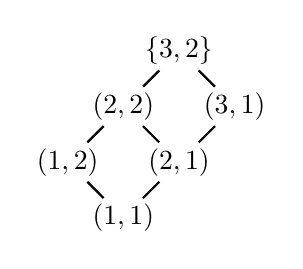
\begin{tikzpicture}
    % First, locate each of the nodes and name them
    \node (top) at (0,0) {$\{3,2\}$};
    \node [below left  of=top] (left)  {$(2,2)$};
    \node [below right of=top] (right) {$(3,1)$};
	\node [below left  of=left] (lleft)  {$(1,2)$};
    \node [below right of=left] (rright) {$(2,1)$};
    \node [below right of=lleft] (last) {$(1,1)$};
    % Now draw the lines:
    \draw [black,  thick, shorten <=-2pt, shorten >=-2pt] (top) -- (left);
    \draw [black, thick, shorten <=-2pt, shorten >=-2pt] (top) -- (right);
    \draw [black,  thick, shorten <=-2pt, shorten >=-2pt] (left) -- (lleft);
    \draw [black, thick, shorten <=-2pt, shorten >=-2pt] (left) -- (rright);
\draw [black, thick, shorten <=-2pt, shorten >=-2pt] (right) -- (rright);
\draw [black, thick, shorten <=-2pt, shorten >=-2pt] (last) -- (lleft);
\draw [black, thick, shorten <=-2pt, shorten >=-2pt] (last) -- (rright);
\end{tikzpicture}\end{center}
\subsubsection{Some Denotions}
\begin{itemize}
\item A Singleton is a set containing only one element.
\item $P(A) = \{B:B\subseteq A\}$
\item $A\triangle B = \{A\cup B\} \setminus \{A\cap B\}$
\item $|\R|=c=\beth_1=\aleph$
\item $A^c = \{b:b \notin A\}$
\item $\prod_{i\in I}{X_i} = \{f:I\to\bigcup_{i\in I}X_i|\forall i\in I(f(i)\in X_i)\}$
\item A pairing function is a bijection $\pi:\N\times\N\to\N$
\item The indicator function of $A\subseteq X$ is $1_A(x)=I_A(x)=\chi_A(x)=1 \iff x$ is in $A$ and equals $0$ otherwise
\end{itemize}
	
	
\end{document}